\documentclass[border=6pt]{standalone}
\usepackage{amsmath,amssymb}\usepackage{tikz}\usetikzlibrary{positioning,arrows.meta,calc}
\begin{document}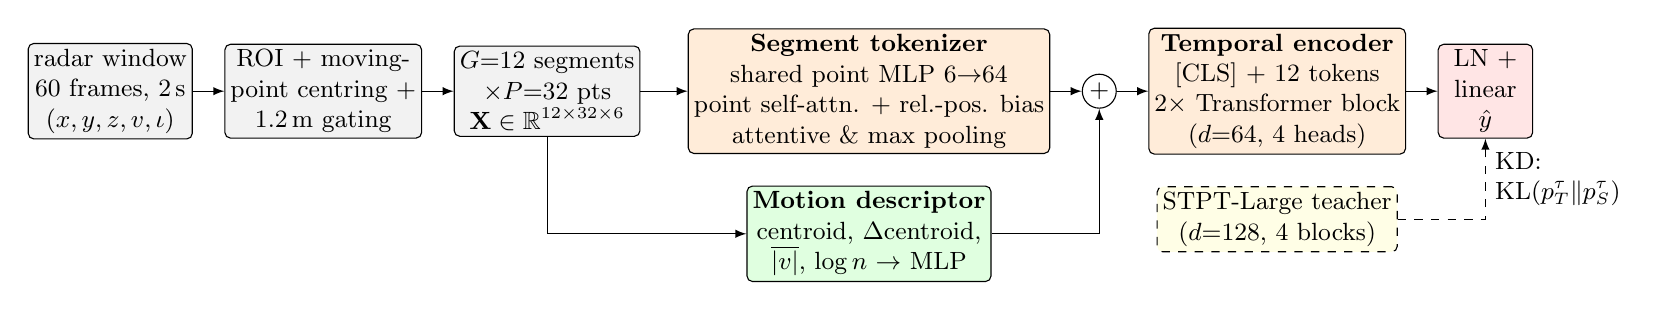
\begin{tikzpicture}[
  font=\small, >=latex,
  box/.style={draw, rounded corners=2pt, align=center, minimum height=7mm, inner sep=2pt},
  frozen/.style={box, fill=blue!8},
  train/.style={box, fill=orange!15},
  mot/.style={box, fill=green!12},
  ]
\node[box, fill=gray!10, minimum width=17mm] (in) {radar window\\$60$ frames, $2$\,s\\$(x,y,z,v,\iota)$};
\node[box, right=4mm of in, minimum width=19mm, fill=gray!10] (pre) {ROI + moving-\\point centring +\\$1.2$\,m gating};
\node[box, right=4mm of pre, minimum width=16mm, fill=gray!10] (seg) {$G{=}12$ segments\\$\times P{=}32$ pts\\$\mathbf{X}\in\mathbb{R}^{12\times32\times6}$};
\node[train, right=6mm of seg, minimum width=26mm] (tok) {\textbf{Segment tokenizer}\\shared point MLP $6{\to}64$\\point self-attn. + rel.-pos. bias\\attentive \& max pooling};
\node[mot, below=4mm of tok, minimum width=26mm] (md) {\textbf{Motion descriptor}\\centroid, $\Delta$centroid,\\$\overline{|v|}$, $\log n$ $\to$ MLP};
\node[circle, draw, right=4mm of tok, inner sep=1pt] (plus) {$+$};
\node[train, right=4mm of plus, minimum width=24mm] (tem) {\textbf{Temporal encoder}\\$[\mathrm{CLS}]$ + 12 tokens\\$2\times$ Transformer block\\($d{=}64$, 4 heads)};
\node[box, right=4mm of tem, minimum width=12mm, fill=red!10] (out) {LN +\\linear\\$\hat{y}$};
\draw[->] (in) -- (pre); \draw[->] (pre) -- (seg); \draw[->] (seg) -- (tok);
\draw[->] (seg.south) |- (md.west); \draw[->] (tok) -- (plus); \draw[->] (md.east) -| (plus.south);
\draw[->] (plus) -- (tem); \draw[->] (tem) -- (out);
\node[box, dashed, below=4mm of tem, minimum width=24mm, fill=yellow!10] (teach) {STPT-Large teacher\\($d{=}128$, 4 blocks)};
\draw[->, dashed] (teach.east) -| node[pos=0.75, right, align=left]{KD:\\$\mathrm{KL}(p_T^{\tau}\Vert p_S^{\tau})$} (out.south);
\end{tikzpicture}\end{document}